%-------------------------------------------------------------------------------
% * MSV Report Class Template and Documentation
\documentclass[oneside]{msvreport}%
% - msvreport is an extension of the standard report class and passes
%   all options to report
% - default options are as in report class with exception of a4paper,
%   openright, and 11pt
% - msvcommon package is loaded and provides TUM color definitions,
%   logos, etc
%
%-------------------------------------------------------------------------------
% ** Options for msvreport (default options are marked (*))
% 1) boolean options for msvreport class:
%  | rmheads (*)    | use roman for headlines and contents                     |
%  | sfheads        | use sans-serif for headlines and contents                |
%  | chapterprefix  | print Chapter prefix in first chapter page               |
%  | bwchapters (*) | print chapter names in black                             |
%  | bluechapters   | print chapter names in blue                              |
%  | headrule       | print horizontal line in header                          |
%  | widetext (*)   | use a wide text body                                     |
%  | narrowtext     | use a narrow text body                                   |
%  | cmyk (*)       | use CMYK colors optimized for printing                   |
%  | print          | alias for cmyk                                           |
%  | rgb            | use RGB colors optimized for monitors                    |
%  | lores (*)      | use low-resolution TUM Banner                            |
%  | hires          | use high resolution TUM Banner                           |

%
% 2) Key/Value options for msvreport class
%  - coverstyle=(none|bw|banner|flags)
%    | none (*) | do not generate cover page                                               |
%    | color    | use color style for cover page                                           |
%    | bw       | use black/white style for cover page (eg for printing on colored covers) |
%    | banner   | use simple banner without flags for cover page (deprecated)              |
%    | flags    | use TUM flag banner for cover page (deprecated)                          |
%
%  - titlestyle=(flags|none|bw|banner)
%    same as coverstyle but for title page
%
%  - copyright=(none|cover|title)
%    | none (*) | do not print copyright notice           |
%    | cover    | print copyright notice after cover page |
%    | title    | print copyright notice after title page |
%
%
%-------------------------------------------------------------------------------
% ** MSV Font Package
% - Standard MSV Report fonts are Times for text and Computer Modern for maths
% - Use option timesmath to enable Times font also in math mode (only pdftex)
% - Do not use msvfonts package if you want to use your own fonts
% - Note that msvfonts loads amsmath package
%
\usepackage{msvfonts}
%
% *** Options for msvfonts
% 1) boolean options for msvfonts package:
% | timestext (*) | use times font for text                                        |
% | fancytext     | use garamond font for text                                     |
% |             +-+                                                                |
% | cmrmath (*) | use computer modern font for text and operators in math-mode     |
% | timesmath   | use times font for text and operators in math mode               |
% |             |   WARNING: timesmath in LuaLaTeX uses unicode-math, which does   |
% |             |   not support the bm package. Use \symbfit and \symbf instead.   |
%
%
% -------------------------------------------------------------------------------
% ** Input Encoding
% - utf8x is recommended at MSV
% - Some comments on encoding can be found here:
%   https://groups.google.com/forum/?fromgroups=#!msg/comp.text.tex/4LC-xODb-LU/1Bd5UZOMNM4J
%
\ifxetexorluatex
  % XeTeX and LuaTeX support utf8 by default
\else
  % File encoding utf8x
  \usepackage{ucs}
  \usepackage[utf8x]{inputenc}
\fi
%
%--------------------------------------------------------------------------------
% ** Language Settings and Hyphenation Patterns
%
% Note: final argument to babel sets the main language
%
\ifxetex%
  \usepackage{polyglossia}
  \setmainlanguage{english}
  \setotherlanguage{german}
%  \setmainlanguage{german}
%  \setotherlanguage{english}
\else
  \usepackage[ngerman,english]{babel} 
\fi
%
%--------------------------------------------------------------------------------
% ** Custom Preamble
% - Start your custom preamble here
% - Use the space before \begin{document} to
%   - Load packages \usepackage{...}
%   - Define custom math operators (DeclareMathOperator)
% - Everything else (including newcommands) starts
%   below \begin{document}

% Here is a list of commonly used packages
% | amsmath   | Many useful tools for typesetting mathematics        |
% | amssymb   | Loads symbol fonts for mathematics, eg \mathbb       |
% | amsthm    | \newtheorem,\theoremstyle commands etc               |
% | thmtools  | Some advanced options for theorem customization      |
% | mathtools | Many useful tools for typesetting maths      |
% | bm        | Bold math (Warning: use only if bold fonts available |
% | algorithm | Tools to typeset algorithms                          |
% | booktabs  | Nice looking tables                                  |
% | enumerate | Enumerated lists                                     |
% | subfig    | Subfigures with common caption                       |
% | caption   | Control caption font                                 |
% | relsize   | Some useful relative font size commands              |
% | xspace    | Control white space after abbreviations              |
% | csquotes  | Quotations according to language selection           |

%-------------------------------------
% random.sty: for sans-serif math fonts
% use with:
%   \usepackage[greek,ngerman,english]{babel}
% does not work with 'timesmath' option in msvfonts
%
\usepackage{bm}
\usepackage{amsmath}
\DeclareMathOperator*{\argmin}{argmin}
\DeclareMathOperator*{\argmax}{argmax}
\newcommand{\norm}[1]{\left\lVert#1\right\rVert}

\usepackage{tikz}
\usetikzlibrary{arrows.meta, calc}

\usepackage{caption}
\usepackage{subcaption}
\usepackage{capt-of}


\newcommand{\B}[1]{\boldsymbol{#1}}
\newcommand{\Bhat}[1]{\boldsymbol{\hat{#1}}}
\newcommand{\e}[1]{\emph{#1}}


\begin{document}
%--------------------------------------------------------------------------------
% ** Custom Commands
% Put your \newcommand's here or \input them from a file
%
%
%--------------------------------------------------------------------------------
% ** Title and Author Information
%
\title{Invertible Neural Networks for MIMO Detection}
\author{Jonas Maas}

\msvdoctype{Bachelor Thesis}

\msvcovertext{%
Supervisor: Univ.-Prof.\ Dr.-Ing.\ Wolfgang Utschick\\[1.5em]
Submission: Xxx xx, 20XX
}

%--------------------------------------------------------------------------------
% ** Title Page
%
\frontmatter
\maketitle
%
%--------------------------------------------------------------------------------
% ** Optional: Abstract
%
\begin{abstract}
There is a lot of recent interest in \emph{Invertible Neural Networks} for density estimation. The idea is to use the architecture of these networks for MIMO Detection. The advantage of this approach is that it does not require the use of complex methods at the receiver to reconstruct the signal. We simply run the received signal through the network in reversed direction. The network is based on \emph{Normalizing Flows} to guarantee the invertability, where the scale and translation variables are learned with the help of \emph{Convolutional Neural Networks} (CNNs).\\ We achieved very good results for low dimensionality but the system is too complex to expand it to high dimensionality at the moment.
\end{abstract}
%
%--------------------------------------------------------------------------------
% ** Table of Contents
%
\tableofcontents
%
%
%--------------------------------------------------------------------------------
% ** First Chapter
%
\mainmatter
\chapter{Introduction}
One of the main topics of communication technology is to reconstruct data at the receiver that was transmitted over a non-trivial channel.\\ \emph{Multiple-Input-Multiple-Output} (MIMO) Detection describes the case where we have multiple transmitter signals, multiple antennas, multiple receiver signals, multiple receiver antennas, etc. The data is transferred over the channel between the transmitter and receiver. In order to reconstruct the original data at the receiver, it is necessary to invert the distortion and the noise, caused by the channel. Over the years many different methods were proposed and used. Recently a lot of researchers tried to use \emph{Neural Networks} for this yet challenging problem. The standard way of using \emph{Neural Networks} for this task is to map the received signals $\B{y}$ to the transmitted signals $\B{x}$. The idea of doing this, is to simplify the transmitter. It is only necessary to feed the trained network with the received signal $\B{y}$ and it then computes the original signal $\B{x}$.\\ We tried a different approach. The transmitted signals $\B{x}$ are mapped to the received signals $\B{y}$ in the natural way and then the origial signals are reconstructed by inverting this mapping in the online phase. The mapping is done with the help of invertible and composable transformations. Afterwards a ML Detector is simply used on each stream and so the NP-hardness is avoided in the real-time system.\\Therefore a network is being used, which is structured into sequential and invertible blocks, where each block is a transformation and has its own \emph{Convolutinal Neural Network}. The internal Networks are used to determine the weights for the affine, autoregressive transformations.


\chapter{Background}
First of all it is essential to outline basic properties of the network and to define the underlying MIMO system.
\section{Channel setup}
The MIMO System consists of $n$ transmitter and $n$ receiver antennas. Each antenna sends a \e{QPSK} signal, thus we have $4^n$ different signals $\B{x}$. 
\begin{equation}
	\B{x} \in \{ \pm \frac{1}{\sqrt{2}} \pm \frac{j}{\sqrt{2}} \}^n
\end{equation}
These signals are transmitted over an \emph{Additive White Gaussian Noise} (AWGN) channel. In this model the signal $\B{x} \in \mathbb{C}^n$ is multiplied with the channel matrix $\B{H} \in \mathbb{C}^{n \times n}$ and then the noise $\B{n} \in \mathbb{C}^n$ is added. The resulting receiver signal is $\B{y} \in \mathbb{C}^n$.

\begin{center}
\begin{tikzpicture}
  \tikzstyle{network} = [rectangle, draw, minimum height = 15mm, minimum width = 20mm, line width = 0.3mm]
  \tikzstyle{sign} = [circle, draw, line width = 0mm]
  
  \node (a) at (0, 0) {$\B{x}_j$};
  \node[network] at (3, 0) (b) {$\B{H}$};
  \node at (6, 0) (c) { \huge $\oplus$};
  \node (d) at (9, 0) {$\B{y}_j = \B{Hx}_j + \B{n}_j$};
  \node[] at (6, 2) (e) {$\B{n}_j \sim \mathcal{N}_C(0, \sigma^2)$};

  \draw[->, line width = 0.3mm] (a) to (b);
  \draw[->, line width = 0.3mm] (b) to (5.77, 0);
  \draw[->, line width = 0.3mm] (6.23, 0) to (d);
  \draw[->, line width = 0.3mm] (e) to (6, 0.23);

\end{tikzpicture}
\end{center}

\noindent Without loosing generality, the channel is assumed to only consist of line-of-sight paths and the structure of the transmitter and receiver to be the same. Then there are direct paths from each transmitter antenna to the associated receiver antenna and some distorted paths from one receiver antenna to the other ones. These paths are added together and result in the following structure
\begin{equation}
	\B{H} = \sum_{k = 1}^K h_k \B{a}(\theta_k)\B{a}(\theta_k)^H, \qquad \B{a}(\theta_k) = [\alpha_k^0 \quad \alpha_k^1 \quad ... \quad \alpha_k^{n-1}]^T, \qquad \alpha_k = e^{-j\pi \sin{\theta_k}}.
\end{equation}
Where $\theta_k$ and $h_k$ are channel specific parameters and are responsible for the magnitude and the shift at the receiver.\\ When having a closer look at one of the receiver antennas, which is represented by one row in the $\B{y}$ vector, the composition of the received signal becomes very clear. 
\begin{equation}
  y_{j,i} = h_{i + 1 , 1} x_{j,0} + h_{i + 1, 2} x_{j,1} + ... + h_{i + 1, i + 1} x_{j,i} + ... + h_{i + 1, n} x_{j, n-1} + n_{j, i}
\end{equation}
There is one summand containing the signal of the corresponding transmitter antenna and the others summands are the damped signals of the other transmitter antennas or noise. We are interested in the, in general, dominating summand of the corresponding transitter antenna. The challenge is to invert the interference and predict the original signal.

\section{Transformations}
\subsection{Inversion of Neural Networks}
The approach of detecting signals by learning the channel and inverting it afterwards requires an \emph{Invertible Neural Network}. Indeed every \emph{Feed-Forward Neural Network} with any bijective activation function is invertible, if the weight matrix is not singular.
\begin{equation}
\begin{split}
  & \B{y} =f(\B{Wx} + \B{b}) \qquad \Leftrightarrow \qquad \B{x} = \B{W}^{-1}(f^{-1}(\B{y}) - \B{b}) \\& \quad  \text{with} \qquad \B{W} \in \mathbb{C}^{n \times n}, \B{b} \in \mathbb{C}^n.
\end{split}
\end{equation}
In this equation $\B{W}$ is the weight-matrix, $\B{b}$ is the bias vector, $\B{x}$ is the input signal and $f$ is the activation function.\\ The problem is the expense and the numerical instability of the inversion. The larger the network, the smaller the elements of the weight matrix, which causes numerical instability. The requirements for the network, we want to build ,are contrary to these problems. The goal is to avoid complexity and errors, caused by the inversion, in the online phase.\\ The idea is to use an \e{Invertible Neural Network} based on simple and composable transformations. Every transformation has to be bijectice with a simple inversion but still has to be capable of learning a highly nonlinear mapping.
\begin{equation}
  \B{z} = T(\B{u}) \qquad \Leftrightarrow \qquad \B{u} = T^{-1}(\B{z}), \qquad \text{with} \qquad \B{z}, \B{u} \in \mathbb{C}^n.
\end{equation}
Such transformations are called \emph{diffeomorphisms}. They are invertible, composable, differentiable and are often used in density estimation tasks. There they have to be differentiable to compute \e{Jacobian matrices}. For our problem it is only assumed that they are invertible and composable.\\ Given two of these transformations $T_1$ and $T_2$, their composition $T_2 \circ T_1$ is also invertible
\begin{equation}
  (T_2 \circ T_1)^{-1} = T_1^{-1} \circ T_2^{-1}.
\end{equation}
Consequently multiple instances of simple tranformations can be composed without loosing invertability. This allows us to construct complex functions out of very simple ones. Each function $T_k$ transforms $\B{z}_{k-1}$ into $\B{z}_k$, assuming $\B{z}_0$ is the input and $\B{z}_K$ is the target.
\begin{equation}
  T = T_K \circ ... \circ T_1 \qquad \text{with} \qquad \B{z}_k = T_k(\B{z}_{k-1})
\end{equation}
Regarding the problem of learning the channel, these transformations allow us to use simple components as a base and combine them. The result is a system that is able to represent a complex mapping without loosing the ability of a simple inversion.

\newpage
\subsection{Affine transformation}
The most simple transformations are affine transformations.
\begin{equation}
  T_i(z_i, \B{h}_i) = \alpha_iz_i + \beta_i \qquad \B{h}_i = \{\alpha_i, \beta_i\} \label{eq:2.8}.
\end{equation}
Equation \ref{eq:2.8} descibes a scaling and a location transformation. The $\alpha_i$ controls the scale of the input and $\beta_i$ determines the location. To guarantee invertability $\alpha_i$ must not be zero $(\alpha_i \neq 0)$. This can be achieved by defining $\alpha_i$ the following way: $\alpha_i = \exp(\tilde{\alpha_i})$. Since $\exp(\cdot)$ can not become zero the invertability of the transformation is guaranteed. \\There are a lot of ways to implement the \e{conditioner} $\B{h}_i$. For this task  each parameter $\tilde{\alpha_i}$ and $\beta_i$ is learned by a seperate \e{Neural Network}.\\ This causes linear growth in complexity with an increasing number of composed transformations. In fact we should be aware of using as little as possible of these transformations.


\subsection{Related Work}
The underlying concept defined above relates to the work in distribution estimation. Especially affine transformations were used a lot in popular papers on this subject, like \emph{non-linear independent components estimation (NICE)}, \textit{real non-volume preserving flow (Real NVP)}, \emph{masked autoregressive flow (MAF)} and \emph{Glow} ~\cite{DBLP:journals/corr/DinhSB16, dinh2014nice, DBLP:journals/corr/KingmaSW16, papamakarios2017masked}. As shown in these papers the networks constructed are based on these transformations and scaled very good. When comparing the underlying problem of all of these networks to the one coverred in this thesis, one finds a lot of similarities. So if you are interested in knowing more about the subject, it's highly recommended to read these papers. More information and much more complex approaches about the transformations itself are covered in \emph{normalizing flows for probabilistic modeling and inference} ~\cite{papamakarios2019normalizing}.

\chapter{Problem specification}
\section{Project goal}
As initially described, there are $4^n$ different signals when using \e{QPSK} and $n$ receiver and transmitter antennas. The signals get transferred over the \e{AWGN channel}, which leads to distorted and noisy signals at the receiver. \\One of the main goals of signal processing is to invert the distortion and noise to get the best possible estimation of the original signal. The upper-bound of this operation can be defined the following way, assuming the use of a trivial channel, whose channel matrix is the identity matrix. In other words, there is no distortion, thus $\B{y} = \B{x} + \B{n}$. It is not possible to get any better, because every signal is separated from each other and there is no way of controlling the noise $\B{n}$ . In this case, the ML-detector can be obtained as
\begin{equation}
\Bhat{x}_j = \argmin_{\B{x}_m} \norm{\B{x}_m - \B{y}_j} \qquad \text{with} \qquad \B{y}_j = (\B{x}_j + \B{n}_j),
\end{equation}
where $\B{x}_j$ is the transmitted signal, $\B{n}_j$ the noise added to the signal and $\B{x}_m$ is one of the $4^n$ possible signals. The goal is to get as close as possible to the upper-bound.


\section{Approach}
Recently a lot of work has gone into the idea of using \emph{Neural Networks} for {MIMO Detection}.\\ 
The basic idea is to map the signal $\B{y}$ to the originial signal $\B{x}$. These networks replace the classical filter structures by trying to learn the inversion of the channel. When using \e{Neural Networks} for detection, the complexity of the receiver can be reduced by simply using the pre-trained network and not having to use complex filters to transform the data. The network gets trained offline with pairs of samples $(\B{y}_j; \B{x}_j)_{j = 1}^{J}$ and then in the online phase the network sees samples of $\B{y}$, it has never seen before and tries to compute the corresponding $\B{x}$.\\ 
Lately \emph{Invertible Neural Networks} have been a subject of high interest, especially in distribution estimation. They are typically used to transform a simple base distribution, like the \emph{Gaussian}, into a target distribution of which only samples are available. This is done by learning the mapping with the help of the networks to be able to invert it afterwards and get more samples of the target distribution.\\
In this paper it is tried to use the same principle for \e{MIMO-Detection}. Instead of mapping $\B{y}$ to $\B{x}$ we try to connect them in the natural way. The idea of mapping $\B{x}$ to $\B{y}$ is to avoid the normally much more complex inverse mapping. Indeed it is not avoided completely, because in the actual detection phase the inverse is used to reconstruct the original signal. However this is done by inverting the system built based on easy transformations and these transformations are very simple to invert. A comparison with the \e{Invertible Neural Networks for density estimation} at hand points out a lot of similarities. We also want to learn a mapping of input data $\B{x}$ to the target data $\B{y}$ with only a limited amount of samples provided. Furthermore the inverse transformation is applied to the received data $\B{y}$ to get back the transmitted data $\B{x}$.\\ 

\noindent When now trying to learn the mapping between $\B{x}$ and $\B{y}$ the following problem is encountered. The signal $\B{x}$ is part of a discrete set and the signal $\B{y}$ is a continuous variable. A bijective function between those two variables is therefore impossible. Considering this, the idea is to map $\B{x} + \B{n}$ to $\B{y}$ with the help of \e{affine diffeomorphisms}. Then the input and target data are continous and the problem is solved at the expense of complexity. The proposed mapping is highly non-linear and there is no formal proof that the transformations used are universal approximators, like discussed in ~\cite{papamakarios2019normalizing}. \\However, in this case simulations took proof of the capability.

\begin{center}
\begin{tikzpicture}
  \tikzstyle{network} = [rectangle, draw, minimum height = 15mm, minimum width = 20mm, line width = 0.5mm]
  
  \node (a) at (0, 0) {$\B{x}_j + \B{n}_j$};
  \node[network] at (4, 0) (b) {INN};
  \node (c) at (8, 0) {$\B{Hx}_j + \B{n}_j$};

  \draw[->, line width = 0.5mm] (a) to (b);
  \draw[->, line width = 0.5mm] (b) to (c);

\end{tikzpicture}
\end{center}
Another advantage is that the only information we need to know about the channel is a finite amount of samples. There is no need to know the channel matrix itself or what type of channel it is used. The architecture of the network is independent of the architecture of the channel.

\begin{center}
\begin{tikzpicture}
  \tikzstyle{network} = [rectangle, draw, minimum height = 15mm, minimum width = 20mm, line width = 0.5mm]
  
  \node (a) at (0, 0) {$\Bhat{x}_j$};
  \node[network] at (3, 0) (b) {Singlestream ML};
  \node[network] at (7, 0) (c) {$\text{INN}^{-1}$};
  \node (d) at (11, 0) {$\B{y}_j = \B{Hx}_j + \B{n}_j$};

  \draw[->, line width = 0.5mm] (d) to (c);
  \draw[->, line width = 0.5mm] (c) to node [above] {$\Bhat{x}_{\text{estim}, j}$} (b) ;
  \draw[->, line width = 0.5mm] (b) to (a);

\end{tikzpicture}
\end{center}
In conclusion the approach can be described as follows. The idea is to train an \emph{Invertible Neural Network} to be able to map $\B{x} + \B{n}$ to $\B{y}$. For this purpose bijective transformations are used to afterwards being able to invert the mapping. When detecting, we receive the signal $\B{y}_j$ and want to get an estimation for the original signal $\B{x}_j$. Therefore the signal $\B{y}_j$ is used as input for the system, which outputs $\Bhat{x}_{\text{estim}, j}$ by inverting the transformations. $\Bhat{x}_{\text{estim}, j}$ gets further processed to receive $\Bhat{x}$, which is one of the $4^n$ signals again. This is done by a \emph{Singlestream-ML}, which is a less complex version of a standard \emph{ML-Detector}. Its use is another benefit of the proposed network. The exact working routine and the advantage of this type of ML is discussed in chapter \ref{Detection}.

\section{Setup for the learning phase}
In the learning phase, we use sets of finite amounts of samples of our actual system to learn the mapping. The learning phase is split into 3 parts, the training phase, the validation phase and the test phase. Every phase uses a different and disjunct set of samples.
\begin{equation}
\begin{split}
	\{ (\B{x}_{j, tr} + \B{n}_{j, tr}, \B{y}_{j, tr})\}^{N}_{j = 1} & \cap \  \{ (\B{x}_{j, val} + \B{n}_{j, val}, \B{y}_{j, val})\}^{M}_{j = 1} \\ &\cap  \{ (\B{x}_{j, test} + \B{n}_{j, test}, \B{y}_{j, test})\}^{L}_{j = 1} = \varnothing.
\end{split}
\end{equation}
Training samples are used to determine the weights and biases of the network. Validation samples are used to compare the performance and avoid overfitting in the training phase. Test samples are used to benchmark the overall performace of the trained network in comparison to other networks. A commonly used segmentation is 60-20-20 in favour of the training samples. Our learning process does not contain the actual test of the inversion while training. It is all about fitting the input data to the target data and trying to find a balance between performance and overfitting in order to get a function as smooth as possible without large deviations.


\chapter{Invertible Neural Network for MIMO Detection}
\section{Main structure of the Invertible Neural Network}
\label{main_structure}
To sum things up till this point, the concept of the forward path can be described as follows. We try to learn a highly nonlinear mapping by combining affine transformations, whose parameters are learned with the help of \e{Neural Networks}. In the beginning it was pointed out, that these very simple transformations need to be coupled with each other to be capable of representing such complex mappings.\\ 

\noindent To do so the system is structured into $K$ sequential blocks, where each block contains an affine transformation and the output of one block is the input of the next block. By doing this the overall transformation is obtained like described above, $T_{total} = T_K \circ ... \circ T_1$. Inside the blocks, the set of parameters $\{\alpha_i, \beta_i\}$ for the transformation needs to be determined. This is where the actual intelligence of the system comes to play. The parameters are determined by a \e{Deep Neural Network}, where each block and each paramter has its own network. The reason for doing this is to avoid correlations of the individual parameters between each other. On the other hand there has to be a solution for the quick increase of complexity. While training, each block that is added, consequents in more networks and therefore $m + o$ more parameters to be determined. $o$ and $m$ represent the complexity of the networks to compute $\alpha$ and $\beta$. Thus it appears that there is a tradeoff between complexity and accuracy, like in almost every technical application. Another problem is that an increasing number of blocks causes error propagation. The more sequential blocks, the more room for error and chance of propagating it through the entire system. There are plenty of options where the errors come from. In our system the most problems are caused by numerical instability. When increasing the number of blocks, one consequence is that inevitably the weights of the network shrink.
\begin{equation}
\begin{split}
  \B{y} = T(\B{x} + \B{n}) = \B{\alpha}_K \odot \B{x}_{K - 1} + \B{\beta}_K & = \B{\alpha}_K \odot (\B{\alpha}_{K - 1} \odot \B{x}_{K - 2} + \B{\beta}_{K-1}) +\B{\beta}_K  \\ & = \B{\alpha}_K \odot \B{\alpha}_{K - 1} \odot \B{x}_{K - 2} + \B{\alpha}_K \odot \B{\beta}_{K-1} + \B{\beta}_K \\ & = ...,
\end{split}
\end{equation}
 where $\odot$ is the \e{Hadamard product} or \e{element-wise product}. With shrinking weights, the fixed data type can become a problem, because the accuracy may not be sufficient enough. Another issue is the correlation of the weights. When changing one weight the whole transformation is changed which in fact requires a lot of fine tuning and optimization. Again the balance between the achievable complexity of the network and the error propagation has to be found.\\
 Inside each block there are two paths, the \textit{forward} and the \textit{backward} path. The forward path is used in the actual training phase to determine the parameters of the network. This path represents the natural way of mapping $\B{x + n}$ to $\B{y}$ and is therefore the actual forward transformation. The backward path on the other hand is used in the online-phase to invert the received signals. It transforms the received signal $\B{y}$ in an estimation for the original signal $\B{x}$ and represents the inverse transformation. Both paths work the exact same way. The input data gets pre-processed in order to then serve as the input of the two \e{Neural Networks} to determine the transformation parameters $\{\alpha_i, \beta_i\}$. The parameters are used to transform the input data $z_i$ into the output data $z_{i+1}$ on the forward path and to transform the input data $z_{i + 1}$ into the output data $z_{i}$ on the inverse path.

\begin{center}
\begin{tikzpicture}
  \tikzstyle{block} = [rectangle, rounded corners, draw, fill=gray!20, minimum height = 70mm, minimum width = 60mm, line width = 0.3mm]
  \tikzstyle{a_block} = [rectangle, rounded corners, draw, fill=gray!20, minimum height = 70mm, minimum width = 22mm, line width = 0.3mm]
  \tikzstyle{network} = [rectangle, rounded corners, fill=blue!60, draw, minimum height = 10mm, minimum width = 20mm, line width = 0.3mm]
  \tikzstyle{variables} = [rectangle, fill = green!80, draw, line width = 0.3mm]
  \tikzstyle{sign} = [circle, fill = yellow!80, draw, line width = 0.3mm]
  \tikzstyle{arrow} = [->, line width = 0.2mm]

  
  \node [variables] at (0,2.7) (input) {$z_i$};
  \node [block] at (4,0) (main){};
  \node [network] at (2.5, 1.5) (network_alpha) {NN};
  \node [network] at (5.5, 1.5) (network_beta) {NN} ;
  \node [variables] at (2.5, -0.5) (alpha) {$\alpha_i$};
  \node [variables] at (5.5, -0.5) (beta) {$\beta_i$};
  \node [sign] at (4, -2.7) (multiply) {$\times$};
  \node [sign] at (5.5, -2.7) (add) {$+$};
  \node [a_block] at (11,0) (i+1){Block $i+1$}; 
  \node [variables] at (8.45,2.7) (output) {$z_{i+1}$};

  \node at (0, 0) {...};
  \node at (13.1, 0) {...};

  \draw[arrow] (0.45,2.7) to (0.95,2.7);
  \draw[arrow] (1.1,2.7) -| (network_alpha);
  \draw[arrow] (2.5,2.7) -| (network_beta);
  \draw[arrow] (network_alpha) to (alpha);
  \draw[arrow] (network_beta) to (beta);
  \draw[arrow] (4, 2.7) to (multiply);
  \draw[arrow] (alpha) |- (multiply);
  \draw[arrow] (multiply) to (add);
  \draw[arrow] (beta) to (add);
  \draw[arrow] (add) to (6.95, -2.7);
  \draw[-, line width = 0.2mm] (7.05, -2.7) to (7.55, -2.7);
  \draw[arrow] (7.55, -2.7) |- (output);
  \draw[arrow] (output) to (9.85, 2.7);
  \draw[arrow] (12.15, -2.7) to (12.5, -2.7);
\end{tikzpicture}
\captionof{figure}{Structure of the system}
\end{center}


\noindent Unlike most other \e{Neural Networks} it does not make a huge difference to compute its parameters on a GPU. The reason is that the network is not very parallel at all. The sequential structure requires sequential computing. In other words we have to handle one block after another, which is the opposite of a parallel structure thus it is not necessary to run the system on GPUs.

\section{Coupling Layers}
The following concept was first proposed in the paper ~\cite{ardizzone2018analyzing}. Like most of the other concepts used, its origins are in density estimation and is modified to apply it on to signals. \\
Each of the sequential structured blocks explained in section ~\ref{main_structure} is a \e{Coupling Layer}. The extension compared to the way we looked at these blocks until now is the technique used to pre-process the input data. Instead of transforming all of the input data, now only parts of the input is transformed and the rest is being run through the block without modifying it.

\begin{center}
\begin{tikzpicture}
  \tikzstyle{block} = [rectangle, rounded corners, draw, fill=gray!20, minimum height = 90mm, minimum width = 60mm, line width = 0.3mm]
  \tikzstyle{a_block} = [rectangle, rounded corners, draw, fill=gray!20, minimum height = 90mm, minimum width = 22mm, line width = 0.3mm]
  \tikzstyle{network} = [rectangle, rounded corners, fill=blue!60, draw, minimum height = 10mm, minimum width = 20mm, line width = 0.3mm]
  \tikzstyle{variables} = [rectangle, fill = green!80, draw, line width = 0.3mm]
  \tikzstyle{sign} = [circle, fill = yellow!80, draw, line width = 0.3mm]
  \tikzstyle{arrow} = [->, line width = 0.2mm]

  
  \node [variables] at (0,3.7) (input) {$z_i$};
  \node [block] at (4,0) (main){};
  \node [network] at (4, 2.5) (filter) {Filter};
  \node [network] at (2.5, 0.5) (network_alpha) {NN};
  \node [network] at (5.5, 0.5) (network_beta) {NN} ;
  \node [variables] at (2.5, -1.5) (alpha) {$\alpha_i$};
  \node [variables] at (5.5, -1.5) (beta) {$\beta_i$};
  \node [sign] at (4, -3.7) (multiply) {$\times$};
  \node [sign] at (5.5, -3.7) (add) {$+$};
  \node [a_block] at (11,0) (i+1){Block $i+1$}; 
  \node [variables] at (8.45,3.7) (output) {$z_{i+1}$};

  \node at (0, 0) {...};
  \node at (13.1, 0) {...};

  \draw[arrow] (0.45,3.7) to (0.95,3.7);
  \draw[arrow] (1.1,3.7) -| (filter);
  \draw[-, line width = 0.2mm] (filter) to (4,1.5);
  \draw[arrow] (4,1.5) -| (network_alpha);
  \draw[arrow] (4,1.5) -| (network_beta);
  \draw[arrow] (network_alpha) to (alpha);
  \draw[arrow] (network_beta) to (beta);
  \draw[arrow] (4, 1.5) to (multiply);
  \draw[arrow] (alpha) |- (multiply);
  \draw[arrow] (multiply) to (add);
  \draw[arrow] (beta) to (add);
  \draw[arrow] (add) to (6.95, -3.7);
  \draw[-, line width = 0.2mm] (7.05, -3.7) to (7.55, -3.7);
  \draw[arrow] (7.55, -3.7) |- (output);
  \draw[arrow] (output) to (9.85, 3.7);
  \draw[arrow] (12.15, -3.7) to (12.5, -3.7);
\end{tikzpicture}
\captionof{figure}{Structure of a \e{Coupling Layer}}
\end{center}

\noindent To get this done, a binary mask $\B{b} \in \{0, 1\}^n$ is applied to the input data of each block. The mask gets generated randomly by distributing a special amount of ones across a zero-vector. The randomness is required to make sure every dimension of the input is transfomed at least once along its path through the system. In other words the unchanged dimensions are exchanged in every other block. \\Another way of making sure to vary the transformed dimensions is to always transform the same dimensions inside one block but to apply \e{permutations} onto the data between several blocks.  \\

\noindent When looking at the special case used for the simulations, it needs at least six layers to make sure every entry of the input vector gets processed together with every other entry in the input vector. The six sequential layers are the lower-bound. But to consider the randomness caused by the generation of the masks and the fact that the mapping is very complex it is necessary to add some more blocks to make sure every input is transformed more than once. \\

\noindent The use of this type of pre-processing routine does not affect the invertability. The forward and the backward paths are still very similar, which is good because we want our backward path to be computable as fast as possible.

\begin{equation}
\begin{split}
  \B{y} & = \B{b} \odot \B{x} + (1-\B{b}) \odot (\B{x} \odot \exp(s(\B{b} \odot \B{x})) + t(\B{b} \odot \B{x})) \\
  \B{x} & = \B{b} \odot \B{y} + (1-\B{b}) \odot (\B{y} - t(\B{b} \odot \B{x}) \odot \exp(-s(\B{b} \odot \B{x})))
\end{split}  
\end{equation}

\noindent $s(\cdot)$ and $t(\cdot)$ stand for the scale and translation. Note that computing the inverse path does not require the invertability of the functions $s(\cdot)$ and $t(\cdot)$. This means the whole non-linearity can be realized with the help of these two variables. In this approach both of these variables are computed with the help of \e{Convolutional Neural Networks}, which are highly nonlinear. \\ Like explained above, each \e{Coupling Layer} transforms a part of the input data and all of the layers are combined together to learn the channel.

\newpage
\section{Internal Neural Networks for parameter determination}
Every block in the sequential structure contains two \e{Neural Networks} to determine the parameters for the transformation. The networks are the most important part of the system and are responsible for good results.\\ 

\noindent The problem can be addressed in two different ways. \\
First of all it can been seen as a regression task, which means the task is to map $\B{x} + \B{n}$ to $\B{y}$ as close as possible. For regression problems the most popular and most common networks are \e{Feed-Forward Networks}. These networks contain alternately a linear transformation followed by a non-linear activation function and was the first approach. The results were not very good, because it seemed like the approach was not complex enough.\\
The other way to look at the problem is to see it as a classification problem. When doing classification, normally the goal is to find clusters in the input data and map them to the pre-defined labels. From this perspective our problem could be seen as mapping $4^n$ clusters to $4^n$ distorted clusters, which represent the labels. $n$ denotes the number of antennas. \\
Classification uses completely different networks but also completely different loss-functions in the training phase. These loss-functions are based on determination of the likelihood of the input data belonging to each of the pre-defined labels. Such loss-functions can not be used, because the network is trained to then be able to run the received data through the inverse network in its natural form. That means the label of the received data is not known. If it was, the problem would be solved already. Instead, we want to be able to use the actual received data and run it through the network without any pre-processing routine.\\
This leads to a mixture of regression and classification. The network itself works on the base of a classification network but the loss function remains a regression one.\\ 
In image classification, which is obviously a classical classification task, most networks are \e{CNNs}. These networks are known for their ability of being able to find structures in pictures. For our input data we use \e{1D-Convolutional Neural Networks} to detect clusters and, in consequence, determine the paramters for the transformations.\\

\begin{figure}
  \centering
  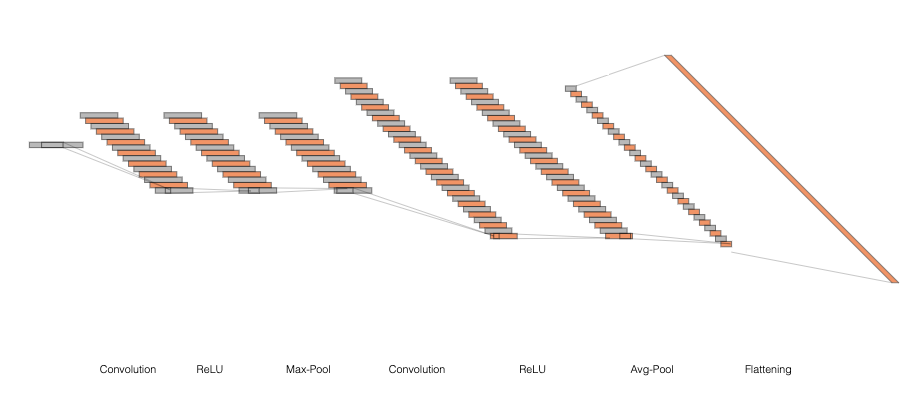
\includegraphics[scale=0.4]{structure_CNN.png}
  \caption{Architecture of the CNN for determination of the parameters $\{\alpha_i, \beta_i\}$}
  \label{fig:structure_CNN}
\end{figure}

\noindent The structure of our network is shown in Figure ~\ref{fig:structure_CNN}. First of all a \e{Convolutional Layer} is applied to the pre-processed input data of each block. Like explained above the convolution tries to find a pattern in the input data. Next a non-linear activation function is applied to the data, followed by a \e{Max-Pooling Layer}. Like in every other network the non-linearity of the activation function is the actual intelligence of the network and the \e{Max-Pool operation} is used to filter the important information and to restrict the complexity. The same structure is applied twice with the difference that instead of the \e{Max-Pool operation} an \e{Average-Pool operation} is applied the second time. Following this the network scaled even better. Afterwards the data gets flattened and further processed by a \e{Feed-Forward Neural Network} and brought in the right shape to calculate the transformation. In the network we are using \e{Dropout Layers}, to make the network more robust and to prevent the network from overfitting. This concept was proposed in ~\cite{hinton2012improving} and is a commonly used technique in machine learning.\\ An observation made while training the network was, that if more channels are used in the \e{CNN} than there are different signals, the system scaled very good. As you can see the system itself is very complex, which supports the initial assumption of a highly non-linear mapping.

\chapter{Detection}\label{Detection}
The purpose of the whole system is to simplify the detection of the signal at the receiver. To do this, nearly every receiver uses a \e{ML-Detector}, which solves the following optimization problem
\begin{equation}
  \Bhat{x}_{ML} = \argmax_{\B{x}} f_{\bm{X}}(\bm{y}; \bm{x}).
\end{equation}
The optimizer searches for the signal $\B{x}$, which maximizes the likelihood that this signal was sent when $\B{y}$ is received. In the case where the channel is an \e{AWGN channel} like here, the equation simplifies to
\begin{equation}
  \Bhat{x}_{ML} = \argmin_{\B{x}} \norm{\B{y} - \B{x}}.
\end{equation}
To solve this optimization problem every possible signal has to be tested and the one with the smallest norm is the one expected to be the best fit. When having \e{QPSK} signals and $n$ antennas, $4^n$ signals have to be tested. Consequently the problem is \e{NP-hard}, which means the complexity of the optimization problem is exponentially growing. If the problem is high-dimensional the detection process gets very costly and will take a lot of time. It has to be accepted that this problem has this large complexity and it is not possible to solve a NP-hard problem exactly with lesser effort.\\

\noindent There are two ways of getting a quicker receiver. The first way is to approximate the solution and to not use the exact solution. The other way is to shift the \e{NP-hardness} away from the receiver. Then the receiver gets faster but on the expense of slowing down some other parts of the system. \\ 
In our approach the \e{NP-hardness} is shifted into the offline learning phase and, in addition, the solution is not exact. This is a consequence of using \e{Neural Networks} for approximating the solution. By doing this  a relatively good solution is obtained and instead of handling the complexity at the receiver it is shifted into the offline training phase. To detect the signal, it is simply ran through the system in the inverse direction.\\ 
The disadvantage of the approach is that we have to deal with the \e{NP-hardness} in the offline phase. In other words the more antennas and the more different signal-points the longer it will take to train the network. The network gets larger because it has to get extended for recognizing more clusters than before. Even the size of the training set increases, when the amount of samples of each signal should maintain the same. In conclusion there is a bigger network with a bigger set of training data which causes an increase in training time.\\
The advantage, on the other hand, is that the detecting process is much more simple. By inverting the channel, there is no more interference between the single dimensions. Thus, the \e{NP-hard} problem is avoided at the detector and a Singlestream-ML can be applied. A \e{Singlestream-ML} is a \e{ML-Detector} which is applied to each dimension alone without taking account of the other dimensions. 
\begin{equation}
  \Bhat{x}_{i, ML} = \argmin_{\B{x}} \norm{\Bhat{x}_{\text{estim},i} - \B{x}_{QPSK}} \qquad i \in \{i \in \mathbb{Z} \ | \ 0 \le i < n\}
\end{equation}
Where $i$ is one of the $n$ dimensions caused by the antennas and $x_{QPSK}$ is one of the $4$ signals transmitted on each stream. Contrary to the ML-Detection explained above the complexity now is only linear in $n$ and not exponential. The complexity could also be seen as constant when considering that the detector can work on each dimension simultaneously. This can be done beacause there is no more interference between the dimensions.\\
In conclusion it can be said that the concept presented in this thesis, has a much faster detecting process with a constant complexity in contrast to the exponential one in standard applications. On the other hand the NP-hardness is shifted into the training phase and with more dimensions it takes much more time to learn the mapping.

\newpage
% \section{Detection on more than one channel}
% The next step is the expansion of the system to be able to work with different channels. Assume there are multiple channels $H_1$, ..., $H_h$,  instead of only one. The channels are all of the type described above, which means there are now multiple channels of the one we peviously used. The difference between the channels are their angles $\alpha_k$ or their weights $h_k$. Data is transmitted over all of the channels and we want a single system that is able to detect the data. The assumptions are like before. The system does not have any information about the channel, it is only trained with samples of all of the channels. The information it has is which channel was used to transmit the signal. 
% \begin{center}
% \begin{tikzpicture}
%   \tikzstyle{network} = [rectangle, draw, minimum height = 15mm, minimum width = 20mm, line width = 0.3mm]
%   \tikzstyle{sign} = [circle, draw, line width = 0mm]
  
%   \node (a) at (0, 0) {$x_i$};
%   \node[network] at (4, 2) (b) {$H_1$};
%   \node[network] at (4, 0) (c) {$H_2$};
%   \node at (4, -1.5) {...};
%   \node[network] at (4, -3) (d) {$H_h$};
%   \node at (9, 0) (e) { \huge $\oplus$};
%   \node (f) at (12, 0) {$y_i$};
%   \node at (9, 2) (g) {$n_i \sim \mathcal{N}_C(0, \sigma^2)$};

%   \draw[-, line width = 0.3mm] (a) to (1.5, 0);
%   \draw[->, line width = 0.3mm] (1.5, 0) |- (b);
%   \draw[->, line width = 0.3mm] (1.5, 0) to (c);
%   \draw[->, line width = 0.3mm] (1.5, 0) |- (d);

%   \draw[-, line width = 0.3mm] (b) -| (6.5, 0);
%   \draw[-, line width = 0.3mm] (c) to (6.5, 0);
%   \draw[-, line width = 0.3mm] (d) -| (6.5, 0);
%   \draw[->, line width = 0.3mm] (6.5, 0) to (8.77, 0);

%   \draw[->, line width = 0.3mm] (g) to (9, 0.23);
%   \draw[->, line width = 0.3mm] (9.23, 0) to (f);

% \end{tikzpicture}
% \end{center}

% Normal receivers have different filters for different channels and for this reason a receiver structure becomes very costly when increasin the numbers of channels.
\chapter{Experiments}
\section{Data Generation}\label{datagen}
The signals we want to transmit are $QPSK$ signals, as described above. These signals are complex natured signals, which leads to the following problem. Most of the toolboxes used for dealing with \e{Neural Networks} are not able to handle complex signals. Therefore it is necessary to transform the signals into a real valued representation. In ~\cite{hellings2019measuring} two transformations were proposed. Here, the first one with the following formula is used.
\begin{equation}
  \bm{\check{x}} = \begin{bmatrix}\Re{(\bm{x})} \\ \Im{(\bm{x})}\end{bmatrix}, \qquad  \bm{\grave{A}} = \grave{\Re}(\bm{A}) = \begin{bmatrix}\Re(\bm{A}) & -\Im(\bm{A}) \\ \Im(\bm{A}) & \Re(\bm{A})\end{bmatrix} 
\end{equation}
In this equation vector $\bm{x}$ and matrix $\bm{A}$ are complex valued. $\bm{\check{{x}}}$ and $\bm{\grave{A}}$ are the real-valued equivalents to the complex valued vector and matrix. \\
The transformation doubles the dimensions of the inputs and thus the complexity increases. Indeed this is no surprise, because each complex valued signal carries two separate information. There is the real part and the imaginary part and both parts contain an information. In fact the transformation gives each information of the complex signal a single real-valued dimension.\\ 
In this case the original signals are two-dimensional which leads to four dimensional input signals for the network. With the approach of two dimensional signals and the use of $QPSK$ there are $16$ different possible signals to transmit. In other words there is a classification task with $16$ different targets or the network has to learn the mapping between $16$ input and $16$ target signals. The reason why we choose to only use such litte dimensionality is, that in the beginning it was not even clear if the approach with invertible neural networks will work. To our knowledge nobody has ever tried such an approach and so the demand of this work was to show the possibilities of this approach.\\ 
In consequence we decided to use very low noise with zero mean and variance of $\frac{1}{5}$. With such little noise the noisy signals are spread around the original data points, without interference between the data points. That means, if applying the ML-Detector on the noisy points, it achieves an accuracy of a hundred percent. The upper bound with a hundred percent is very hard to achieve. \\
The other variables we have to determine are the channel variables. There are the stream-weights $h_k$ and the angles $\theta_k$. We use equal weights which means that each stream has the same power and the same damping. This does not restrict the generality. The angles are also freely selectable. But if you are using \e{supplementary} angles the matrix becomes singular. \e{Supplementary} angles mean that the angles sum up to $180$ degrees. \\
Data generation is done in \e{Matlab} and then the data is converted into the shape the \e{python} network requests it to be. Like described above there are four different data sets for training, validation, testing and for the inverse path. All of these data sets use the same channel and signal parameters but contain different instances.\\
For better scaling of the network the data gets \e{normalized}. This kind of pre-processing routine shifts the whole data into the interval $[-1; 1]$. Here \e{normalizing} is done by searching for the maxima of $\B{x}_i + \B{n}_i$ and then dividing the whole data by the maxima. We are doing this for each dataset on its own. The used approach is the most trivial one and can not handle huge additive noise. Assuming there is a huge noise value $\B{n}_i$ added to the corresponding signal value $\B{x}_i$ in the training data and the other noise values are comparatively little. Then the whole pre-processing routine in this dataset is dominated by the bigger one. This causes irregular distribution of the noisy datapoints over the interval $[-1; 1]$. In the other datasets the distribution is normal, which means the datapoints are spread over the interval regular. Then the network learns some strange mapping and when applying the network on the other data sets it scales poorly. So we have to pay attention to big noise values and in general to noise with big variance when using this approach.\\

\noindent The whole pre-processing routine is done to avoid inputs with large magnitude. If there are inputs with small and big magnitude, the ones with big magnitude have more impact on the weight updates than the other ones. By normalizing them, all inputs have nearly the same impact on the weight updates.
\begin{equation}
  \triangle w_{i} \sim x_i
\end{equation}
The 60-20-20 rule is used to determine how many samples of each signal there are in each data set. These samples are divided into batches, where every batch contains 20 samples. The samples are distributed randomly over the batches, to, in the best case, have one sample of each signal in every batch. We tried to distribute the samples in different orders over the batches but the random distribution worked best. The batches are then used to train the network.

\newpage
\section{Network}
The structure of the system used for detection is described above. We are using sequential \emph{Coupling Layers} with affine transformations to learn the mapping between $\B{x} + \B{n}$ and $\B{y}$. The parameters of the transformations are determined by internal \emph{Convolutional Neural Networks} in the corresponding block.\\

\noindent There are a lot of \emph{hyperparameters} in the system and in this chapter the effect of the most important ones is explained. \\First of all the network has to be initialized. Orthogonal initialization is used. It is popular for the improvement in performance and for a better abilitiy to converge. The effect of orthogonal initialization was profen in \emph{Provable Benefit of Orthogonal Initialization in Optimizing Deep Linear Networks} ~\cite{hu2020provable}.\\

\noindent One of the main \e{hyperprameters} is the number of sequential blocks. The number of blocks represents the number of combined transformations and thereby the complexity of the mapping. We are using $15$ or more blocks to be able to get a system that is complex enough to represent the mapping. With an increasing number of blocks the complexity and consequently the amount of time to learn the networks increases rapidly. At about 30 sequential blocks the positive effect of being able to represent a more complex mapping and the negative effect of propagating errors through the network compensate each other. The best results were achieved when using 15 blocks.\\

\noindent The next parameter worth a more intense study is the amount of hidden units. This number comes to play when talking about the complexity of the \e{Feed-Forward-Network} where the flattened outcome of the \e{Convolutional Neural Network} gets passed to. With the number of hidden units the complexity can be further determined. The disadvantage in increasing the amount of hidden units is the chance to overfit the network. The network looses generality and tries to learn features which are not even there. The best results were achieved with 500 to 700 hidden units.\\

\noindent The architecture of the internal \e{Convolutional Neural Networks}, is very important for the performance of the system. The \e{CNNs} try to find features in the input data and determine the variables of the transformations to recognize them. To get good results, a good choice of its parameters is necessary. There are a lot of internal parameters but we highlight only a few of them. \\
The number of channels made a huge difference in performance. Channels are the result of the convolution operations and represent different features of the input data. This means the more channels the network has the more features it can probably learn. Like said before, an increase in channels makes a huge improvement in the accurancy of the outcome. Especially more channels than different signals scaled very good.\\
Filter size is also worth a mention. It determines the number of input dimensions processed together. The network then tries to find features in those parts of the data. Our approach was to look at as much dimensions as possible at the same time, because each input dimension influences every other target dimension.\\
Other than that there are a lot of other parameters but we have not tried a lot of different configurations regarding them.\\

\noindent A commonly discussed topic when talking about \e{Neural Networks} is the activation function. It is the actual intelligence of the network and there are a lot of options to choose from. In most cases the \e{ReLU}, the \e{sigmoid} or the \e{tanh} function is used. The \e{ReLU} is the most common one for this kind of problem and it also worked best here. Regarding the performance, the difference between the functions were not large but the \e{ReLU} was the most consistent one.\\ 

\noindent The network used, achieved an accurancy of arround $96$ percent in the best case. Due to the statistical component of the network it does not perform the same way on every simulation but varies a bit in performance. However the used \emph{hyperparameters} allowed us to constantly achieve around $95$ percent. In these simulations the system consisted of $15$ sequential blocks, 500 hidden layers, \e{ReLU} activation function, $60$ channels for the first convolutional operation and $120$ channels for the second one.\\

\begin{figure}
\begin{subfigure}{.5\textwidth}
  \centering
  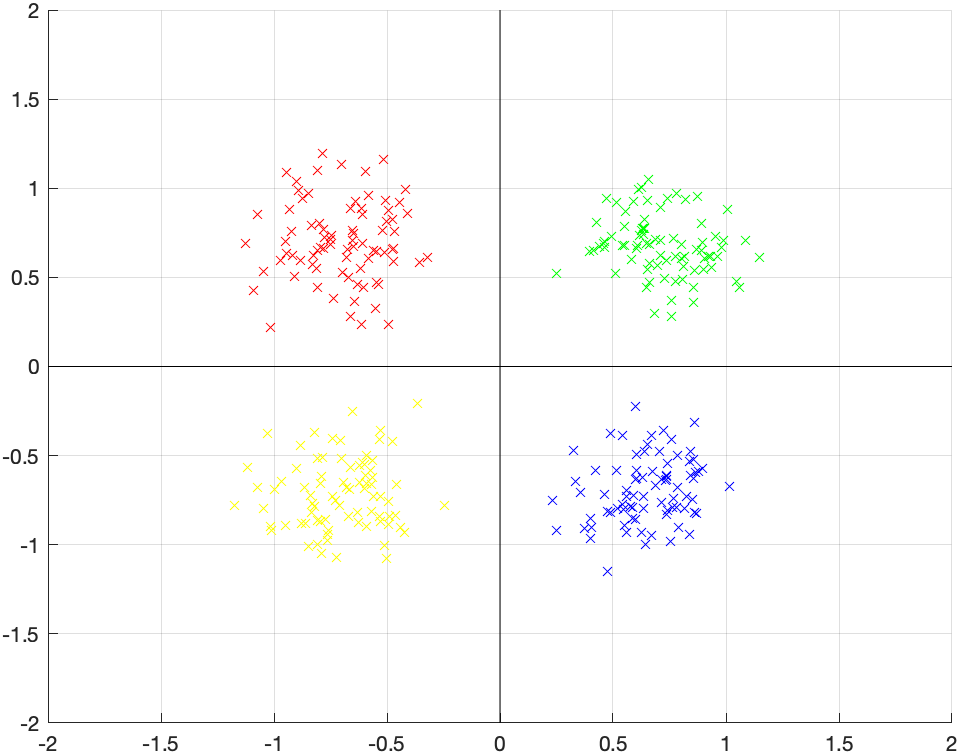
\includegraphics[width=.8\linewidth]{xplusn.png}  
  \caption{$\B{x}_j + \B{n}_j$}
  \label{fig:sub-first}
\end{subfigure}
\begin{subfigure}{.5\textwidth}
  \centering
  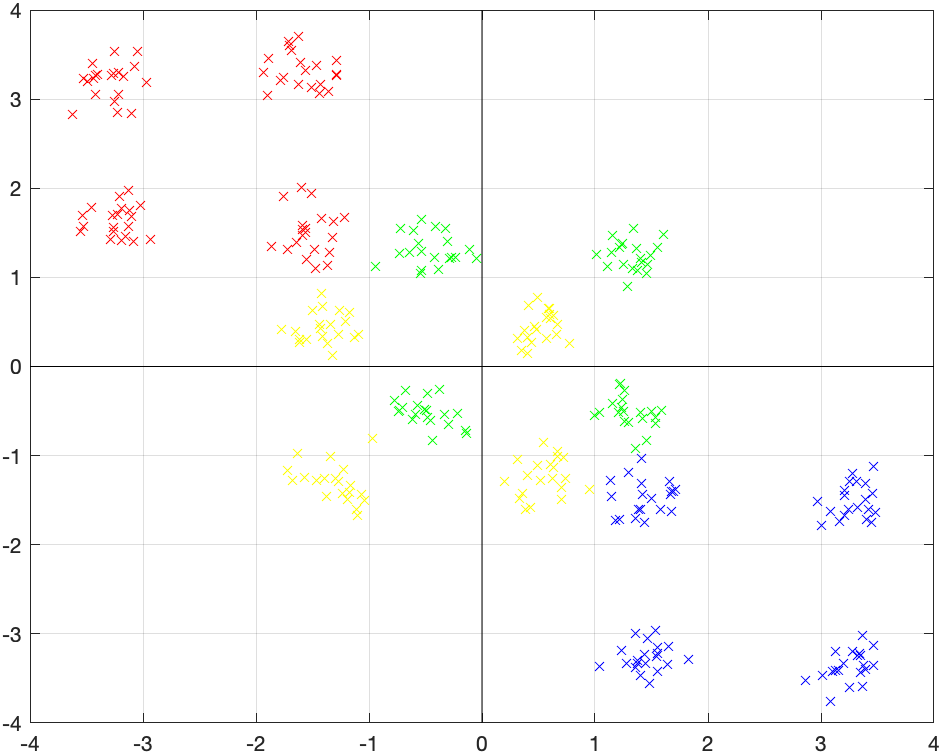
\includegraphics[width=.8\linewidth]{y.png}  
  \caption{$\B{y}_j$}
  \label{fig:sub-second}
\end{subfigure}

% \newline

\begin{subfigure}{.5\textwidth}
  \centering
  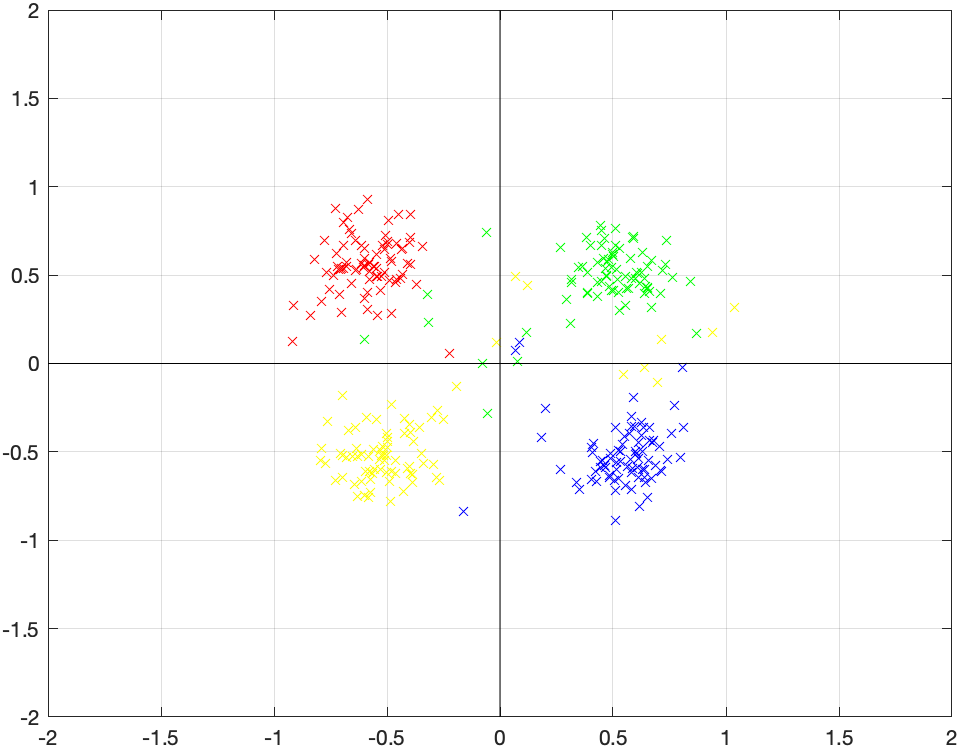
\includegraphics[width=.8\linewidth]{estim.png}  
  \caption{$\B{x}_{\text{estim}, j}$}
  \label{fig:sub-third}
\end{subfigure}
\begin{subfigure}{.5\textwidth}
  \centering
  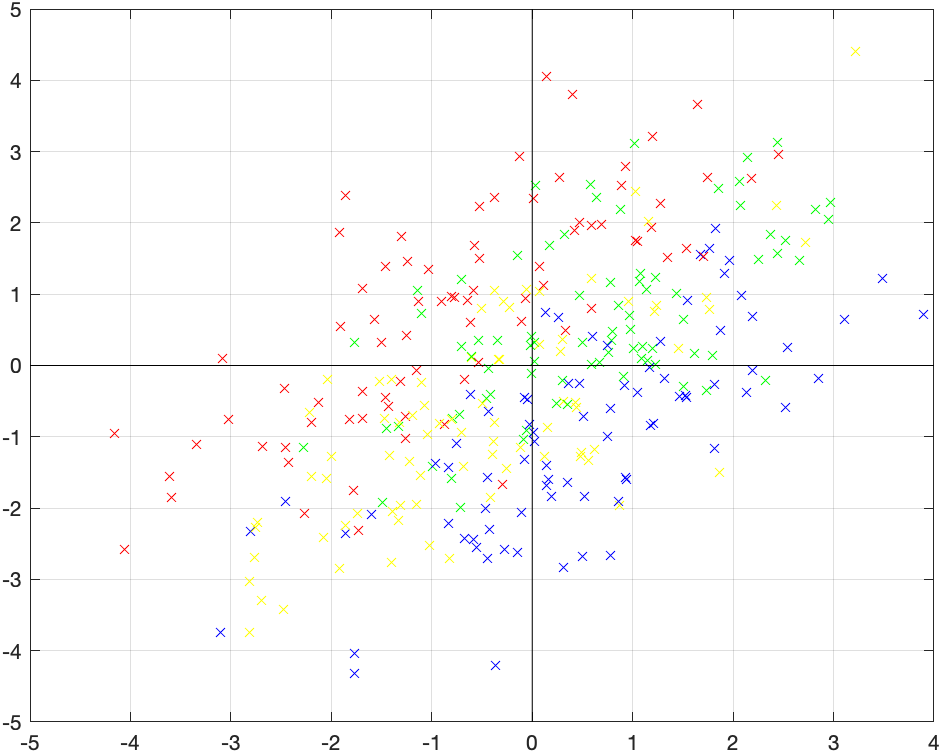
\includegraphics[width=.8\linewidth]{linear.png}  
  \caption{$\B{x}_{\text{linear}, j} = \B{H}^{-1}\B{y}_j$}
  \label{fig:sub-fourth}
\end{subfigure}
\caption{Real part of the signals}
\label{fig:fig}
\end{figure}

\noindent In figure ~\ref{fig:fig} the real-part of both transmitted signals is plotted against each other. The first subplot ~\ref{fig:sub-first} shows the input of the system $\B{x}_j + \B{n}_j$. The four different clusters, caused by the four different real parts, can clearly be seen. The noise is \e{Gaussian} with very small variance. When taking account of the imaginary-parts too, there are $16$ input clusters which have to be mapped to the $16$ target clusters. They can be seen in ~\ref{fig:sub-second}. The yet challenging problem is the adjacency of the target clusters. Some of them are very close to each other which causes a lot of trouble for the network. Especially with a high variance it gets hard for the network to differentiate between the different clusters.\\

\noindent In figure~\ref{fig:sub-third} the actual performance of the network can be seen. The signals plotted are the estimations of the network. Therefore the trained network got the received signal $\B{y}_j$ as an input and the backward path was used to compute an prediction for the transmitted signal $\B{x}_j$. After applying a \e{Singlestream-ML} to the signal $\B{x}_{\text{estim}, j}$ the estimated transmitter signal $\Bhat{x}_j$ is obtained. The plot shows, that the performance of the system is actually very good. Most of the data points got reconstructed very well. The clusters of the estimated signals are even not as spread as the original ones, which means that the network was able to supress parts of the noise. You can also identify a few outliers, especially caused by the yellow and the green signal points. These are the consequence of the mentioned adjacency of these clusters, see subplot~\ref{fig:sub-second}.\\

\noindent Like one would imagine, the \e{channel-matrix} has a huge impact on the distribution of the target clusters. The matrix can be changed by varying the angles $\theta_k$ or the weights $h_k$. With some parameters the clusters are very separated from each other and with others they are very close. A special case is when the \e{channel-matrix} gets singular. The network presented in this chapter was tested with a lot of different combinations and even performed very good on inverting the singular matrix.

\section{Discussion}
In this section we want to compare our results to results of other approaches and then discuss them afterwards.\\

\noindent At first we will have a closer look to the most simple, the linear approach. 

\begin{center}
\begin{tikzpicture}
  \tikzstyle{network} = [rectangle, draw, minimum height = 15mm, minimum width = 20mm, line width = 0.3mm]
  \tikzstyle{sign} = [circle, draw, line width = 0mm]
  
  \node (a) at (0, 0) {$\B{x}_j$};
  \node[network] at (2.5, 0) (b) {$\B{H}$};
  \node at (4.5, 0) (c) { \huge $\oplus$};
  \node[network] at (6.5, 0) (d) {$\B{H}^{-1}$};
  \node[] at (4.5, 2) (e) {$\B{n}_j \sim \mathcal{N}_C(0, \sigma^2)$};
  \node (f) at (10.5, 0) {$\Bhat{x}_j = \B{x}_j + \B{H}^{-1}\B{n}_j$};

  \draw[->, line width = 0.3mm] (a) to (b);
  \draw[->, line width = 0.3mm] (b) to (4.27, 0);
  \draw[->, line width = 0.3mm] (4.73, 0) to (d);
  \draw[->, line width = 0.3mm] (e) to (4.5, 0.23);
  \draw[->, line width = 0.3mm] (d) to (f);


\end{tikzpicture}
\end{center}

\noindent When doing this, the received signal $\B{y}_j$ gets multiplied by the inverse \e{channel-matrix} $\B{H}^{-1}$ to receive the estimation $\Bhat{x}_j = \B{H}^{-1}\B{y}_j$. The result of this operation can be seen in figure 6.1d . As you can see the result was very poor. The detection accuracy was between 30 and 40 percent. In the figure you can see that this operation was not able to reconstruct the original clusters. The linear transformation was not complex enough to get good results. Another disadvantage in comparison to the proposed approach is the missing ability to handle singular or nearly singular \e{channel-matrices}. In this case the linear transformation simply does not work at all.\\

\noindent Like mentioned in the beginning the normal way to use \e{Neural-Networks} for \e{MIMO-Detection} would be to map the received signal $\B{y}$ to $\B{x}$. We want to compare the results of the \e{Invertible Neural Network} to the results of the standard approach. Therefore we used the structure of the best performing network. But instead of using both the forward and backward path, only the forward path was used for the training as well as the detection phase. In the training phase the network tried to learn the mapping between $\B{y}$ and $\B{x}$ and in the detection phase the network got samples it has never seen before and tried to apply the mapping. The results were very bad and very inconsistent in comparisson to the results of the \e{Invertible Neural Network}. It could be concluded that mapping $\B{y}$ to $\B{x}$ is much more complicated than mapping $\B{x} + \B{n}$ to $\B{y}$. There is no formal proof for this assumption but the simulation results validated it, at least for the kind of system we are using.\\

\noindent In summary we have shown that \e{Invertible Neural Networks} are usable for \e{MIMO-Detection}. The proposed network achieved remarkable results and could be improved to achieve state of the art accurancy. However the system has only been tested on low dimensionality. We ran a few simulations with the extension of the system to four antennas. These simulations took proof of the rapidly increasing complexity and in consequence the learning phase was very time consuming. The results were not as good as the ones from the two dimensional system but the system was not optimated yet. \\ To be able to extend the network to higher dimensions without the need of infinite time for the learning phase, we have to find a better structure for the network. The structure should be less complex, to decrease the amount of time the network needs to be trained. On the other hand the structure has to be as capable, regarding the ability to represent a complex mapping, as the structure proposed here. Another way of improving the results is to find a better pre-processing routine without impairing the performance when normalizing. The exact problem is described in section ~\ref{datagen}.\\

\noindent In conclusion it can be said that the approach has a lot of good aspects and is promising. It still needs a lot of optimization to be able to compete against standard systems and it has to be tested if the system is usable for more dimensions.




%--------------------------------------------------------------------------------
% ** Appendix
%
\appendix

\cleardoublepage
% \bibliographystyle{unsrt}
%--------------------------------------------------------------------------------
% ** References 
\bibliographystyle{IEEEtran}
\refstepcounter{chapter}
\addcontentsline{toc}{chapter}{\bibname}
\bibliography{IEEEabrv,references}

% \cleardoublepage
% \refstepcounter{chapter}
% \addcontentsline{toc}{chapter}{\indexname}
% \printindex
% \end{comment}
\end{document}
